\chapter{Conclusions}
\label{chapter:conclusions}
\begin{music}
    \parindent10mm \instrumentnumber{1} \setstaffs1{1} 
    \generalmeter{\meterfrac34} \generalsignature{-1}
    \startextract
		\notes  \en
    \zendextract
\end{music}
\epigraph{\textit{A childish mind will turn to noble ambition}}{Ocarina of Time}

In this thesis we explored the relationship between an organism phenotype and bifurcations in differential equations models seeking to model the organism behaviour. In the collaboration in synthetic biology in chapter \ref{chapter:double-exclusive}, the experimental design goals were to engineer a particular phenotypic behaviour of \emph{E. coli}. This amounted to designing particular bifurcations in the corresponding differential equation model. A gap in machine learning methods for differential equations that optimise with respect to targets directly in state space was identified, leading to the proposed method in Chapter \ref{chapter:inference}. We laid the foundations for methods that learn differential equation models that match qualitative behaviours and high-level constraints. With this new method now in hand, we revisit how the collaboration in synthetic biology would have benefited and propose a \emph{Design-Learn} workflow that we argue would benefit any collaboration which designs phenotypes by iterative genetic manipulation of an organism. Differential equation models for an organism behaviour are not always available, as the collaboration in immunology in chapter \ref{chapter:exploring}. We outlined the importance of interactive exploration and refinement of annotations of high-dimensional data clouds and built \emph{FlowAtlas.jl} to enable immunophenotyping across datasets with heterogeneous experimental designs. Our retrospectives are concluded with a vision of how methods from chapter \ref{chapter:exploring} can be used together with our proposed \emph{Design-Learn} workflow to organise and reduce different models of organisms whose behaviours can be experimentally captured with flow cytometry.

We now discuss the most promising future directions that use this thesis as a starting point, in particular 

\section{Retrospectives}
\subsection{A \emph{Design-Learn} workflow for synthetic biology}

\begin{Figure}
	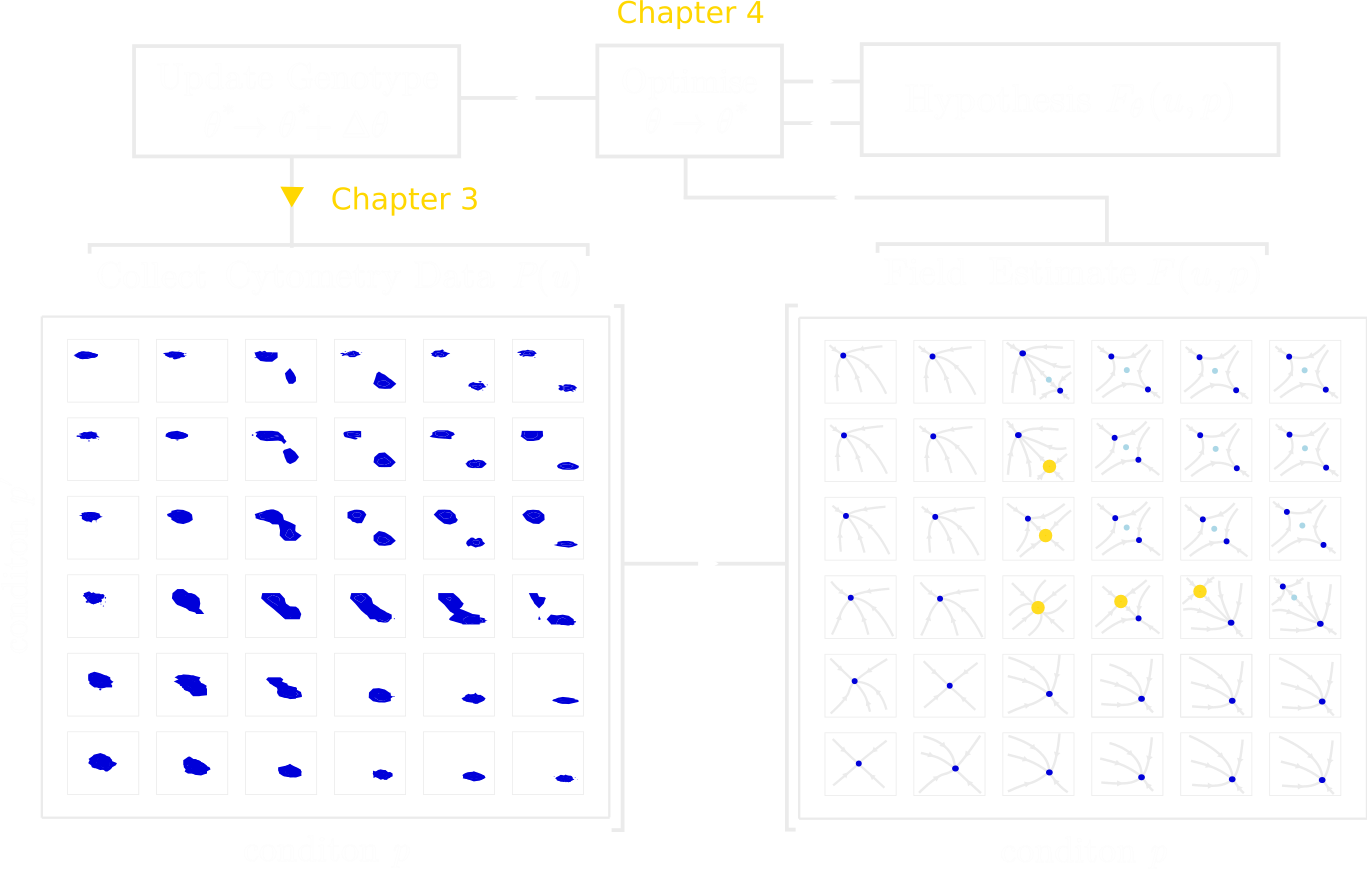
\includegraphics[width=\linewidth]{design-learn}
	\caption{Overview for a \emph{design-learn} workflow, developed in hindsight, for genetic design of the \emph{double exclusive reporter}. Non-parametric estimates of the field $F(u,p)$ yield state space geometry from cytometry data. A parametrised hypothesis $\rates(u,p)$ is then optimised against the data-driven state space geometry, to obtain optimal parameters $\theta^*$. The neighbourhood of $\theta^*$ is then investigated to inform genetic modifications and subsequent collection of more cytometry data.}
	\label{fig:deisgn-learn}
\end{Figure}

\subsection{Bifurcations \& model reduction}


\section{Future Work}

\subsection{Designing Limit Cycles}

\subsection{Spatially Extended Systems}

\section{Limitations \& Alternative Approaches}


\begin{enumerate}
    \item How can thesis results be applied to biological computing \cite{Dalchau2018}
\end{enumerate}